\chapter{Funzioni Termodinamiche}

Dal primo principio della teromidinamica sappiamo che il differenziale dell'energia interna di un sistema può essere scritto come 

\begin{equation}
    dE = \delta Q - \delta L
    \label{primo_princ_termodinamica}
\end{equation}

Dove $Q$ indica il calore e $L$ indica il lavoro. Si usa $\delta$ perché queste due quantità non sono differenziali esatti, in quanto $Q$ e $L$ non sono funzioni di stato ma dipendono dal cammino.\\

Possiamo elaborare la \eqref{primo_princ_termodinamica} in modo che possa tornare più utile per successive elaborazioni. 

Ricordando la definzione di entropia\mkeyword{entropia} si ottiene 

\begin{equation}
    dS = \frac{\delta Q}{T} \implies \delta Q = T \ dS
\end{equation}

Mentre possiamo scrivere qualunque tipo di lavoro come il prodotto fra una forza generalizzata (proprietà intensiva) e uno spostamento generalizzato (quantità estensiva).
Alcuni tipi di lavoro che ci possono tornare utili in questo corso sono riportati in tabella\\

\begin{table}[htbp]
    \centering
    \begin{tabular}{lll}
        \toprule
        Tipo di lavoro & Forza generalizzata & Spostamento generalizzato \\
                       & (intensiva)         & (estensivo) \\
        \midrule
        meccanico    & $F$ (forza)                  & $s$ (spostamento)      \\
        espansivo    & $-P$ (pressione)             & $V$ (volume)           \\
        chimico      & $\mu$ (potenziale chimico)   & $n$ (numero di moli)   \\
        elettrico    & $\phi$ (potenziale elettrico)& $q$ (carica elettrica) \\
        superficiale & $\gamma$ (tensione superficiale) & $\Sigma$ (area della superficie) \\
        \bottomrule
    \end{tabular}
    \caption{Coppie coniugate di variabili termodinamiche.
    Ogni forma di lavoro si scrive come prodotto di una variabile intensiva per il differenziale della corrispondente variabile estensiva, $\delta L = \sum_i Y_i\,dX_i$.}
    \label{tab:coppieconiugate}
\end{table}

Le quantità di gran lunga più importanti sono due: il lavoro espansivo e il lavoro chimico. 

Dato che analizzeremo il caso di reazioni chimiche possiamo scrivere il differenziale del lavoro come 

\begin{equation}
    \delta L = P dV - \sum_{i = 1}^N \mu_i d n_i
\end{equation}

Dove l'indice $i$ si riferisce alle $N$ sostanze coinvolte nella reazione. \\

Il differenziale dell'energia interna su cui lavoreremo da ora in poi sarà quindi:

\begin{equation}
    dE = T dS - P dV + \sum_{i = 1}^N \mu_i d n_i
    \label{differenziale_energia}
\end{equation}

\section{Trasformata di Legendre e funzioni ausiliarie}

Nell'equazione \eqref{differenziale_energia} le quantità presenti in veste di variazioni infinitesime sono entropia, volume e numero di moli. 
Queste quantità sono dette variabili naturali\mkeyword{variabili naturali} dell’energia interna. Le variabili naturali sono quelle variabili da cui la funzione di stato considerata dipende esplicitamente e rispetto a cui risulta più semplice integrare il differenziale in modo da ottenere una espressione della funzione per una particolare trasformazione del nostro sistema.\\

Dalla \eqref{differenziale_energia} e dalla definizione di differenziale possiamo ottenere le espressioni di alcune derivate dell’energia interna:

\begin{equation}
    P = - \left( \frac{\partial E}{\partial V} \right)_{S,n} \quad T = \left( \frac{\partial E}{\partial S} \right)_{V,n} \quad \mu_i = \left( \frac{\partial E}{\partial n_i} \right)_{S,P,j \neq i}
\end{equation}

Nella pratica sperimentale però non è semplice misurare una derivata rispetto al volume o una derivata rispetto all’entropia. \\

Possiamo costruire delle funzioni di stato ausiliarie dell’energia interna che dipendono da altre variabili naturali tramite una operazione chiamata trasformata di Legendre\mkeyword{trasformata di Legendre}. Una trasformata è una operazione che trasforma una funzione (in questo caso in forma di differenziale) in un’altra funzione che dipende da altre variabili ma contiene informazioni sul sistema che descrive equivalenti.

La trasforma di Legendre di un differenziale di una funzione di stato si ottiene sommando a destra e sinistra il differenziale del prodotto di una quantità intensiva e di una quantità estensiva.

Perché una trasformata di Legendre abbia senso e sia utile bisogna che:

\begin{itemize}
    \item Le dimensioni del prodotto della quantità estensiva e della quantità intensiva siano le stesse della funzione. In questo caso un’energia.
    \item La somma sia fatta in modo da semplificare uno dei termini esistenti con uno di quelli sommati (questo per l’utilità).
\end{itemize}

\subsection{Entalpia}

La prima trasformata utile si ottiene sommando a entrambi i membri della \eqref{differenziale_energia} il differenziale del prodotto $PV$, che ha le dimensioni di un'energia come richiesto.
Sviluppando il differenziale del prodotto si ha $d(PV) = P\,dV + V\,dP$, e dunque
\begin{equation}
    dE + d(PV) = T\,dS - P\,dV + P\,dV + V\,dP + \sum_{i=1}^{N}\mu_i\,dn_i ,
    \label{eq:entalpia_passaggio}
\end{equation}
dove i due termini in $P\,dV$ si elidono, che è precisamente la semplificazione richiesta dal secondo criterio.
Poiché il primo membro non è altro che $d(E + PV)$, la funzione di stato così definita
\begin{equation}
    H = E + PV
    \label{eq:def_entalpia}
\end{equation}
prende il nome di entalpia\mkeyword{entalpia}, e il suo differenziale vale
\begin{equation}
    dH = T\,dS + V\,dP + \sum_{i=1}^{N}\mu_i\,dn_i .
    \label{eq:diff_entalpia}
\end{equation}
Il confronto fra la \eqref{eq:diff_entalpia} e la \eqref{differenziale_energia} mostra che cosa la trasformata abbia fatto: ha sostituito il volume con la pressione nell'elenco delle variabili naturali, lasciando invariato tutto il resto.
Il vantaggio pratico è immediato, perché a pressione costante il secondo termine si annulla e, in assenza di reazioni, $dH = T\,dS = \delta Q$: la variazione di entalpia coincide con il calore scambiato, che è la grandezza che un calorimetro misura direttamente.
È questa la ragione per cui i calori di reazione si tabulano come entalpie e non come energie interne.

\subsection{Energia libera di Gibbs}

Applicando all'entalpia una seconda trasformata, questa volta sottraendo il differenziale del prodotto $TS$, si ottiene
\begin{equation}
    dH - d(TS) = T\,dS - T\,dS - S\,dT + V\,dP + \sum_{i=1}^{N}\mu_i\,dn_i ,
    \label{eq:gibbs_passaggio}
\end{equation}
dove stavolta a elidersi sono i due termini in $T\,dS$.
La funzione di stato risultante
\begin{equation}
    G = H - TS = E + PV - TS
    \label{eq:def_gibbs}
\end{equation}
si chiama energia libera di Gibbs\mkeyword{energia libera di Gibbs} e ha differenziale
\begin{equation}
    dG = -S\,dT + V\,dP + \sum_{i=1}^{N}\mu_i\,dn_i .
    \label{eq:diff_gibbs}
\end{equation}
Le sue variabili naturali sono $T$, $P$ e i numeri di moli, cioè esattamente le grandezze che si controllano in un laboratorio: un recipiente aperto immerso in un bagno termostatico è a pressione atmosferica e a temperatura fissata, e non c'è alcun modo diretto di imporre invece un valore dell'entropia.
Ne segue che $G$ è la funzione termodinamica naturale per descrivere le reazioni chimiche, ed è quella su cui lavoreremo nel resto del corso.
Nelle condizioni usuali di $T$ e $P$ costanti la \eqref{eq:diff_gibbs} si riduce infatti a
\begin{equation}
    dG = \sum_{i=1}^{N}\mu_i\,dn_i ,
    \label{eq:gibbs_isotermobarico}
\end{equation}
cioè l'energia libera di Gibbs varia soltanto in conseguenza del procedere della reazione, ed è per questo che il potenziale chimico governerà l'equilibrio.

\newpage

\subsection{Energia libera di Helmholtz}

L'ultima delle quattro funzioni si ottiene applicando direttamente all'energia interna la trasformata rispetto al prodotto $TS$, senza passare per l'entalpia:
\begin{equation}
    dE - d(TS) = -S\,dT - P\,dV + \sum_{i=1}^{N}\mu_i\,dn_i = dA ,
    \label{eq:diff_helmholtz}
\end{equation}
con
\begin{equation}
    A = E - TS .
    \label{eq:def_helmholtz}
\end{equation}
Questa funzione, indicata talvolta con $F$, prende il nome di energia libera di Helmholtz\mkeyword{energia libera di Helmholtz} e ha per variabili naturali $T$, $V$ e i numeri di moli.
Svolge per i sistemi a volume costante lo stesso ruolo che $G$ svolge per quelli a pressione costante, ed è quindi la funzione appropriata per un recipiente rigido e chiuso, come una bomba calorimetrica o una bombola, mantenuto a temperatura costante.\\

Le quattro funzioni non sono indipendenti fra loro ma legate a due a due dalle trasformate appena viste, e conviene raccoglierne i differenziali per confronto:
\begin{align}
    dE &= T\,dS - P\,dV + \sum_i \mu_i\,dn_i , \label{eq:riepilogo_E}\\
    dH &= T\,dS + V\,dP + \sum_i \mu_i\,dn_i , \label{eq:riepilogo_H}\\
    dA &= -S\,dT - P\,dV + \sum_i \mu_i\,dn_i , \label{eq:riepilogo_A}\\
    dG &= -S\,dT + V\,dP + \sum_i \mu_i\,dn_i . \label{eq:riepilogo_G}
\end{align}
Il termine chimico è identico in tutte e quattro, il che riflette il fatto che nessuna delle trasformate ha toccato la coppia coniugata $(\mu_i, n_i)$, e da qui segue che il potenziale chimico si può ottenere derivando indifferentemente una qualunque delle quattro rispetto a $n_i$, purché mantenendo costanti le variabili naturali appropriate.
Si osservi inoltre che $E$ e $H$ hanno l'entropia fra le variabili naturali, mentre $A$ e $G$ hanno soltanto grandezze direttamente controllabili in laboratorio: è questa, e non una maggiore generalità, la ragione della loro utilità pratica.\\

Esiste un trucco per memorizzare le espressioni di questi differenziali noto come quadrato termodinamico\mkeyword{quadrato termodinamico}:

\begin{figure}[htbp]
    \centering
    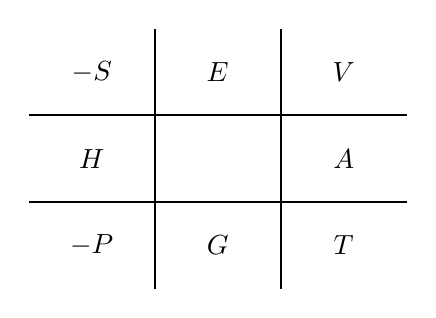
\begin{tikzpicture}
        % --- macro riutilizzabili -----------------------------------------
        \def\cella#1#2#3{\node at (#1,#2) {$#3$};}
        \def\colonna{0.80}   % semilarghezza di una cella
        \def\riga{0.55}      % semialtezza di una cella
        % --- griglia ------------------------------------------------------
        \draw[thick] (-2.40, 0.55) -- (2.40, 0.55);
        \draw[thick] (-2.40,-0.55) -- (2.40,-0.55);
        \draw[thick] (-0.80,-1.65) -- (-0.80,1.65);
        \draw[thick] ( 0.80,-1.65) -- ( 0.80,1.65);
        % --- vertici e lati -----------------------------------------------
        \cella{-1.60}{ 1.10}{-S}
        \cella{ 0.00}{ 1.10}{E}
        \cella{ 1.60}{ 1.10}{V}
        \cella{-1.60}{ 0.00}{H}
        \cella{ 1.60}{ 0.00}{A}
        \cella{-1.60}{-1.10}{-P}
        \cella{ 0.00}{-1.10}{G}
        \cella{ 1.60}{-1.10}{T}
    \end{tikzpicture}
    \label{fig:quadrato}
\end{figure}
 
Ogni funzione di stato è compresa fra le sue variabili naturali. Queste vanno moltiplicate per le grandezze che sono diametralmente opposte. 
In alto sono poste le grandezze estensive (S e V) ed in basso quelle intensive (P e T). S e P (che sono sulla sinistra) hanno segno negativo. Se per andare dalla quantità estensiva a quella intensiva vado da sinistra verso destra il segno è quello risultante dalla moltiplicazione. Altrimenti il segno va invertito.

\section{Relazioni di Maxwell e loro applicazioni}

Consideriamo un sistema a composizione chimica costante ovvero in cui non variano i numeri di moli dei vari componenti, quindi $dn_i = 0 \ \forall i$ . Questo equivale ad annullare il terzo termine sulla destra dell’equazione \eqref{differenziale_energia}. 
Se dividiamo entrambi i termini per $dV$ otteniamo:

\begin{equation}
    \left( \frac{\partial E}{\partial V} \right)_T = T \left( \frac{\partial S}{\partial V} \right)_T - P
\end{equation}

L’equazione contiene una quantità che è complessa da calcolare: la derivata parziale dell’entropia rispetto al volume a temperatura costante.
Infatti non esiste nessun modo per misurare direttamente l’entropia quindi tutte le quantità legate all’entropia non sono semplici da calcolare o misurare. 

Cerchiamo così di sostituire questo termine. 

Consideriamo il differenziale dell'energia libera di Helmoltz:

\begin{equation}
    dA = - SdT - P dV
\end{equation}

Da cui si ottiene facilmente che 

\begin{equation}
    P = - \left( \frac{\partial A}{\partial V} \right)_T \qquad S = -\left( \frac{\partial A}{\partial T} \right)_V
\end{equation}

Applicando il teorma di Schwartz

\begin{equation}
    \frac{\partial}{\partial T}\left( \frac{\partial A}{\partial V} \right)_T = \frac{\partial}{\partial V}\left( \frac{\partial A}{\partial T} \right)_V
\end{equation}

E quindi 

\begin{equation}
    \left( \frac{\partial S}{\partial V} \right)_T = \left( \frac{\partial P}{\partial T} \right)_V
\end{equation}

Allora sostituendo nell'equazione iniziale

\begin{equation}
    \left(\frac{\partial E}{\partial V}\right)_T = T \left( \frac{\partial P}{\partial T} \right)_V - P
\end{equation}

\subsection{Gas ideale}

Per un gas ideale l'equazione di stato fornisce $P = nRT/V$, da cui

\begin{equation}
    \left(\frac{\partial P}{\partial T}\right)_V = \frac{nR}{V} = \frac{P}{T} ,
    \label{eq:derivata_ideale}
\end{equation}

e sostituendo nella relazione appena ricavata si ottiene

\begin{equation}
    \left(\frac{\partial E}{\partial V}\right)_T = T\,\frac{nR}{V} - P = P - P = 0 .
    \label{eq:pressione_interna_ideale}
\end{equation}

La \eqref{eq:pressione_interna_ideale} dice che l'energia interna di un gas ideale non dipende dal volume ma dalla sola temperatura, il che è coerente con il modello microscopico: in assenza di forze fra le molecole non esiste alcuna energia potenziale di interazione, e allontanarle non costa nulla.
Vale la pena osservare che l'implicazione si inverte, poiché l'annullamento della \eqref{eq:pressione_interna_ideale} si realizza soltanto se l'equazione di stato è quella dei gas perfetti: qualunque altra equazione dà un risultato diverso da zero.

\subsection{Gas reale di van der Waals}

Esplicitando rispetto alla pressione l'equazione di van der Waals si ha

\begin{equation}
    P = \frac{nRT}{V - b} - \frac{an^2}{V^2} ,
    \label{eq:vdw_esplicita_cap}
\end{equation}

nella quale il secondo termine non dipende dalla temperatura, cosicché

\begin{equation}
    \left(\frac{\partial P}{\partial T}\right)_V = \frac{nR}{V - b} .
    \label{eq:derivata_vdw}
\end{equation}

Sostituendo si ottiene

\begin{equation}
    \left(\frac{\partial E}{\partial V}\right)_T = \frac{nRT}{V - b} - P = \frac{nRT}{V - b} - \left(\frac{nRT}{V - b} - \frac{an^2}{V^2}\right) = \frac{an^2}{V^2} ,
    \label{eq:pressione_interna_vdw}
\end{equation}

dove si osservi che il covolume $b$ si semplifica e sopravvive la sola costante $a$.
Per un gas reale l'energia interna dipende dunque dal volume, e la quantità \eqref{eq:pressione_interna_vdw}, detta pressione interna\mkeyword{pressione interna}, misura il lavoro necessario per allontanare le molecole vincendo le loro attrazioni reciproche.
Il fatto che compaia $a$ e non $b$ è significativo: a determinare la dipendenza dal volume sono le forze attrattive a lungo raggio discusse nel capitolo sulle interazioni intermolecolari, non l'ingombro sterico, che agisce soltanto sull'equazione di stato.
Coerentemente, la \eqref{eq:pressione_interna_vdw} decresce come $V^{-2}$ e si annulla nel limite di grandi volumi, dove le molecole sono in media abbastanza distanti perché l'attrazione diventi trascurabile e il gas reale tenda a quello ideale.

\subsection{Relazione fra $C_P$ e $C_V$}

Un'ultima applicazione riguarda il legame fra i due calori specifici.
Partendo dalla definizione $C_P = (\partial H/\partial T)_P$ e da $H = E + PV$ si ha

\begin{equation}
    C_P = \left(\frac{\partial E}{\partial T}\right)_P + P\left(\frac{\partial V}{\partial T}\right)_P ,
    \label{eq:cp_primopasso}
\end{equation}

dove compare la derivata dell'energia interna a pressione costante e non a volume costante.
Per collegarla a $C_V$ si scrive il differenziale di $E$ nelle sue variabili $(T,V)$ e lo si valuta lungo un cammino a pressione costante, lungo il quale il volume è funzione della temperatura:

\begin{equation}
    \left(\frac{\partial E}{\partial T}\right)_P = C_V + \left(\frac{\partial E}{\partial V}\right)_T\left(\frac{\partial V}{\partial T}\right)_P .
    \label{eq:catena}
\end{equation}

Sostituendo la \eqref{eq:catena} nella \eqref{eq:cp_primopasso} e raccogliendo si ottiene

\begin{equation}
    C_P - C_V = \left[\left(\frac{\partial E}{\partial V}\right)_T + P\right]\left(\frac{\partial V}{\partial T}\right)_P .
    \label{eq:cp_cv}
\end{equation}

La \eqref{eq:cp_cv} non fornisce un'espressione dei due calori specifici presi singolarmente, ma soltanto della loro differenza: per calcolare $C_P$ o $C_V$ separatamente serve sempre un modello microscopico, come la teoria cinetica dei gas o il modello a oscillatori di Dulong e Petit.\\

Il fattore $(\partial V/\partial T)_P$ quantifica di quanto il sistema si dilata scaldandolo, mentre la parentesi quadra rappresenta l'energia necessaria per unità di dilatazione, con il termine $P$ dovuto al lavoro contro la pressione esterna e il termine $(\partial E/\partial V)_T$ dovuto al lavoro contro le forze intermolecolari.\\

Nel caso del gas ideale entrambi i fattori sono noti, poiché $(\partial E/\partial V)_T = 0$ per la \eqref{eq:pressione_interna_ideale} e $(\partial V/\partial T)_P = nR/P$, e la \eqref{eq:cp_cv} si riduce a

\begin{equation}
    C_P - C_V = P\,\frac{nR}{P} = nR ,
    \label{eq:mayer}
\end{equation}

cioè alla relazione di Mayer, nella quale sopravvive il solo lavoro espansivo.\\

Negli altri casi il calcolo è assai più complicato, ma si possono comunque fare due considerazioni generali.
La prima è che $(\partial E/\partial V)_T > 0$, perché a temperatura costante aumentare il volume di una sostanza richiede sempre di fornire energia, e nessuna porzione di materia cede energia dilatandosi.
La seconda è che $(\partial V/\partial T)_P > 0$, perché a pressione costante aumentare la temperatura di un gas, di un liquido o di un solido ne aumenta il volume.
Essendo positivi entrambi i fattori della \eqref{eq:cp_cv}, si conclude che

\begin{equation}
    C_P - C_V > 0
    \label{eq:disuguaglianza_calori}
\end{equation}

per qualunque sostanza: scaldare a pressione costante costa sempre più energia che scaldare a volume costante, perché parte del calore fornito viene spesa nel lavoro di dilatazione anziché nell'aumento di temperatura.

\section{Il potenziale chimico}

L'energia interna è una grandezza estensiva, e lo sono anche tutte le sue variabili naturali $S$, $V$ e $n_i$: se raddoppiamo il sistema, raddoppiano tutte.
In termini matematici questo significa che $E$ è una funzione omogenea di grado uno,

\begin{equation}
    E(\lambda S, \lambda V, \lambda n_i) = \lambda\,E(S,V,n_i)
    \qquad \forall \lambda > 0 ,
    \label{eq:omogeneita}
\end{equation}

e derivando entrambi i membri della \eqref{eq:omogeneita} rispetto a $\lambda$ e ponendo poi $\lambda = 1$ si ottiene
\begin{equation}
    E = S\left(\frac{\partial E}{\partial S}\right)_{V,n} + V\left(\frac{\partial E}{\partial V}\right)_{S,n} + \sum_{i=1}^{N} n_i \left(\frac{\partial E}{\partial n_i}\right)_{S,V,n_{j\neq i}} ,
    \label{eq:eulero}
\end{equation}
risultato noto come teorema di Eulero\mkeyword{teorema di Eulero} sulle funzioni omogenee.
Poiché le tre derivate sono note dal differenziale dell'energia interna, e valgono rispettivamente $T$, $-P$ e $\mu_i$, la \eqref{eq:eulero} diventa
\begin{equation}
    E = TS - PV + \sum_{i=1}^{N}\mu_i n_i .
    \label{eq:E_integrata}
\end{equation}
Si osservi che questa non è la banale rimozione dei differenziali dall'espressione di $dE$, operazione che sarebbe illecita poiché $T$, $P$ e $\mu_i$ non sono costanti: è una conseguenza dell'estensività, e vale soltanto per essa.

Differenziando la \eqref{eq:E_integrata} come prodotto si ottiene
\begin{equation}
    dE = T\,dS + S\,dT - P\,dV - V\,dP + \sum_{i=1}^{N}\mu_i\,dn_i + \sum_{i=1}^{N} n_i\,d\mu_i ,
    \label{eq:dE_differenziata}
\end{equation}
e il confronto con l'espressione originale di $dE$ mostra che tre termini compaiono in entrambe e si elidono, lasciando
\begin{equation}
    S\,dT - V\,dP + \sum_{i=1}^{N} n_i\,d\mu_i = 0 .
    \label{eq:gibbs_duhem}
\end{equation}
La \eqref{eq:gibbs_duhem} è la relazione di Gibbs-Duhem\mkeyword{relazione di Gibbs-Duhem}, e contiene come variabili soltanto grandezze intensive, cioè $T$, $P$ e i potenziali chimici.
Il suo contenuto è che tali grandezze non sono indipendenti fra loro: determinate tutte tranne una, la mancante resta fissata.

\subsection{Potenziale chimico di un gas ideale}

Applichiamo la \eqref{eq:gibbs_duhem} a un sistema con un solo componente e a temperatura costante, cosicché il primo termine si annulla e resta $n\,d\mu = V\,dP$.
Sostituendo l'equazione di stato dei gas ideali nella forma $V = nRT/P$ si ottiene

\begin{equation}
    d\mu = \frac{V}{n}\,dP = \frac{RT}{P}\,dP ,
    \label{eq:dmu}
\end{equation}

e integrando la \eqref{eq:dmu} fra una pressione di riferimento $P^0$ e la pressione $P$ si ricava

\begin{equation}
    \mu = \mu^0 + RT\ln\frac{P}{P^0} .
    \label{eq:mu_gas}
\end{equation}

La costante di integrazione $\mu^0$ prende il nome di potenziale chimico standard\mkeyword{potenziale chimico standard} ed è il valore assunto da $\mu$ quando la pressione parziale eguaglia quella di riferimento, convenzionalmente $P^0 = 1 \ atm$; il suo valore dipende dalla sola temperatura e dalla scelta dello stato di riferimento.
Si noti che l'argomento del logaritmo è il rapporto fra due pressioni, ed è quindi adimensionale, come dev'essere: scrivere $\ln P$ ha senso solo sottintendendo la divisione per $P^0$ e misurando le pressioni in atmosfere.

\subsection{La costante di equilibrio}

Poniamoci a temperatura e pressione costanti, condizione tipica di un recipiente aperto e termostatato, cosicché il differenziale dell'energia libera di Gibbs si riduce a

\begin{equation}
    dG_{T,P} = \sum_{i=1}^{N}\mu_i\,dn_i .
    \label{eq:dG_TP}
\end{equation}

Se nel sistema avviene una reazione, le variazioni dei numeri di moli non sono indipendenti ma legate ai coefficienti stechiometrici $\nu_i$, positivi per i prodotti e negativi per i reagenti, tramite un unico parametro $\xi$ detto coordinata di reazione\mkeyword{coordinata di reazione}:

\begin{equation}
    dn_i = \nu_i\,d\xi .
    \label{eq:coordinata}
\end{equation}

Sostituendo la \eqref{eq:coordinata} nella \eqref{eq:dG_TP} e dividendo per $d\xi$ si ottiene

\begin{equation}
    \left(\frac{\partial G}{\partial \xi}\right)_{T,P} = \sum_{i=1}^{N}\nu_i\,\mu_i ,
    \label{eq:derivata_xi}
\end{equation}

cioè, a $T$ e $P$ fissate, l'energia libera di Gibbs è funzione della sola coordinata di reazione.

Il criterio di spontaneità segue immediatamente.
Poiché a temperatura e pressione costanti la diminuzione di $G$ misura il lavoro utile che il sistema può produrre, la composizione può evolvere spontaneamente solo verso valori di $\xi$ ai quali $G$ è minore.

\begin{figure}[htbp]
    \centering
    \begin{tikzpicture}[x=2.2cm, y=2.2cm, >={Latex[length=2mm]}]
        % --- macro riutilizzabili -----------------------------------------
        \def\gibbs{0.9*\x-ln(\x)+0.05}
        \def\xA{0.42}      \def\yA{1.296}
        \def\xE{1.111}     \def\yE{0.945}
        \def\punto#1#2#3#4{%
            \fill (#1,#2) circle (1.7pt);
            \node[anchor=#4, font=\small] at (#1,#2) {$#3$};
        }
        \def\richiamo#1#2{\draw[dotted] (0,#2) -- (#1,#2);}
        % --- assi ---------------------------------------------------------
        \draw[->] (0,0) -- (3.35,0) node[below left] {$\xi$};
        \draw[->] (0,0) -- (0,2.00) node[left] {$G$};
        % --- curva --------------------------------------------------------
        \draw[domain=0.28:3.00, samples=200, smooth, thick] plot (\x, {\gibbs});
        % --- linee di richiamo --------------------------------------------
        \richiamo{\xA}{\yA}
        \richiamo{\xE}{\yE}
        % --- variazione di energia libera ---------------------------------
        \draw[<->] (0.16,\yE) -- (0.16,\yA);
        \node[anchor=west, font=\small] at (0.20,1.12) {$\Delta G$};
        % --- punti notevoli -----------------------------------------------
        \punto{\xA}{\yA}{A}{south west}
        \punto{\xE}{\yE}{E}{south west}
    \end{tikzpicture}
    \caption{Energia libera di Gibbs in funzione della coordinata di reazione, a temperatura e pressione costanti.}
    \label{fig:gibbs_xi}
\end{figure}

La reazione procede dunque finché $G$ diminuisce, e si arresta quando raggiunge il minimo, dove la derivata si annulla:

\begin{equation}
    \left(\frac{\partial G}{\partial \xi}\right)_{T,P} = \sum_{i=1}^{N}\nu_i\,\mu_i = 0 .
    \label{eq:condizione_equilibrio}
\end{equation}

La \eqref{eq:condizione_equilibrio} è la condizione di equilibrio chimico, e va letta con attenzione: l'equilibrio non corrisponde all'esaurimento dei reagenti, ma a un minimo di $G$ che cade in generale a un valore intermedio di $\xi$.

Sostituendo ora nella \eqref{eq:condizione_equilibrio} l'espressione \eqref{eq:mu_gas} del potenziale chimico si ottiene
\begin{equation}
    \sum_{i=1}^{N}\nu_i\,\mu_i^0 + RT\sum_{i=1}^{N}\nu_i \ln\frac{P_i}{P^0} = 0 ,
    \label{eq:equilibrio_sostituito}
\end{equation}
dove i $P_i$ sono le pressioni parziali all'equilibrio.
La prima sommatoria è una combinazione di costanti tabulate e si definisce energia libera di Gibbs standard di reazione\mkeyword{energia libera standard di reazione},
\begin{equation}
    \Delta G^0 = \sum_{i=1}^{N}\nu_i\,\mu_i^0 ,
    \label{eq:deltaG0}
\end{equation}
mentre la seconda si compatta usando le proprietà dei logaritmi, poiché $\nu\ln A = \ln A^{\nu}$ e $\ln A + \ln B = \ln(AB)$:
\begin{equation}
    \sum_{i=1}^{N}\nu_i \ln\frac{P_i}{P^0} = \ln \prod_{i=1}^{N}\left(\frac{P_i}{P^0}\right)^{\nu_i} = \ln K_P .
    \label{eq:def_KP}
\end{equation}
La quantità $K_P$ così definita è la costante di equilibrio\mkeyword{costante di equilibrio} riferita alle pressioni parziali; poiché i coefficienti dei reagenti sono negativi, essi finiscono automaticamente a denominatore, e per una reazione del tipo $aA + bB \rightarrow cC + dD$ si ha esplicitamente
\begin{equation}
    K_P = \frac{(P_C/P^0)^{c}\,(P_D/P^0)^{d}}{(P_A/P^0)^{a}\,(P_B/P^0)^{b}} .
    \label{eq:KP_esplicita}
\end{equation}
Sostituendo la \eqref{eq:deltaG0} e la \eqref{eq:def_KP} nella \eqref{eq:equilibrio_sostituito} si ottiene infine
\begin{equation}
    \Delta G^0 + RT\ln K_P = 0 ,
    \qquad\text{ovvero}\qquad
    \Delta G^0 = -RT\ln K_P ,
    \label{eq:equazione_fondamentale}
\end{equation}
che è l'equazione fondamentale dell'equilibrio chimico.
Il suo interesse pratico è considerevole: i potenziali chimici standard di moltissimi composti sono stati misurati e tabulati, quindi la \eqref{eq:equazione_fondamentale} permette di prevedere la composizione all'equilibrio di un gran numero di reazioni senza eseguirle.

Va sottolineato che tutta la derivazione poggia sulla \eqref{eq:mu_gas}, ricavata assumendo il comportamento di gas ideale, e vale quindi rigorosamente solo per reazioni fra gas in condizioni non troppo lontane dall'idealità.\\

Un'espressione formalmente identica si applica però alle specie diluite in soluzione, per le quali si pone
\begin{equation}
    \mu = \mu^0 + RT\ln\frac{[C]}{c^0} ,
    \label{eq:mu_soluzione}
\end{equation}
con $c^0 = 1 \ mol/L$ come concentrazione di riferimento, e la costante di equilibrio diventa
\begin{equation}
    K_C = \frac{[C]^{c}[D]^{d}}{[A]^{a}[B]^{b}} ,
    \label{eq:KC}
\end{equation}
sempre intendendo le concentrazioni divise per $c^0$.
La sostituzione si giustifica osservando che una soluzione diluita e un gas ideale condividono la proprietà essenziale, cioè che le molecole di soluto sono abbastanza distanti fra loro da poter trascurare le interazioni reciproche, esattamente come le molecole di un gas rarefatto.